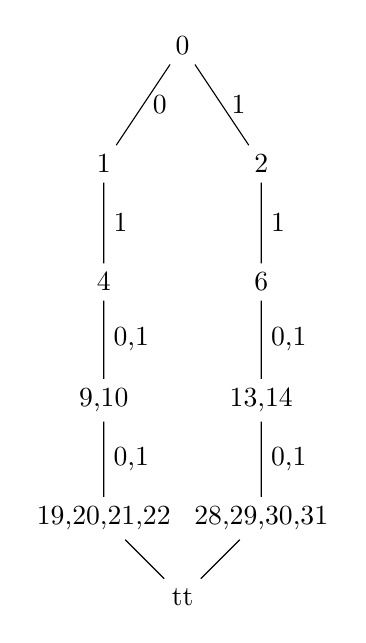
\begin{tikzpicture}
  [
    level 1/.style = {sibling distance = 2cm},
  ]

  \node (root) at (0,0) {0}
  child {node {1}
      child {
          node {4}
          child {node {9,10}
              child {node {19,20,21,22}
                  edge from parent node [right] {0,1}}
              edge from parent node [right] {0,1}}
          edge from parent node [right] {1}}
      edge from parent node [right] {0}
    }
  child {node {2}
      child {node {6}
          child {node {13,14}
              child {node {28,29,30,31}
                  edge from parent node [right] {0,1}}
              edge from parent node [right] {0,1}}
          edge from parent node [right] {1}}
      edge from parent node [right] {1}
    };

  \node (bottomnode) at (0,-7) {tt};

  \foreach \w in {1,2}{
      \draw (root-\w-1-1-1) -- (bottomnode);
    }

\end{tikzpicture}